\documentclass[20pt,a1paper,landscape,blockverticalspace=-0.25in]{tikzposter}
\usepackage[utf8]{inputenc}
\usepackage{csquotes}
\usepackage{amsmath}
\usepackage{amsfonts}
\usepackage{amsthm}
\usepackage{amssymb}
\usepackage{mathrsfs}
\usepackage{graphicx}
\graphicspath{{./images/}}
\usepackage{adjustbox}
\usepackage{enumitem}
\usepackage{xcolor}
\usepackage{tartu}
\usepackage[comma]{natbib}
\usepackage{har2nat}
\bibliographystyle{agsm}
\setcitestyle{citesep={;}}
\renewcommand{\bibsection}{}
\setlength{\bibsep}{0pt}

% set theme parameters
\tikzposterlatexaffectionproofoff
\usetheme{UniTartuTheme}
\usecolorstyle{UniTartuStyle}

\usepackage[scaled]{helvet}
\renewcommand\familydefault{\sfdefault} 
\renewcommand{\vec}[1]{\bm{#1}}
\newcommand{\Tr}{\text{Tr}}
\usepackage[T1]{fontenc}

\title{Bayesian Inference of Parameters for Numerical Storm Surge Models}
\author{\textbf{Benjamin Russell}\textsuperscript{1}}
\institute{\textsuperscript{1}University of Durham\\}
\titlegraphic{
\includegraphics[width=0.12\linewidth]{logo.png}}

% begin document
\begin{document}
	\maketitle
	\centering
	\begin{columns}
		\column{0.32}
		\block{Background}{
			In the United States of America coastal communities suffer huge yearly losses from flooding. One of the causes of such flooding is storm surges, this is the sea level rise caused by tropical hurricanes and cyclones. Studies have shown that between 1963 and 2012 49\% of all deaths from hurricanes in the US were caused by the storm surge(Fig. \ref{fig:deaths})~\cite{deaths}. The economic impact has also been huge with estimates showing that with no further improvements to coastal flood defenses by 2050 yearly losses from storm surge flooding could exceed US\$1trillion~\cite{costs}.
			
			Following this it makes sense to model and simulate these storm surge events to facilitate better planning for flood defence spending. Most storm surge models require finely tuned parameters which either require direct measurement which can be expensive and difficult to carry out or to be inferred from previous data. Inferrence of these parameters requires huge numbers of time consuming model runs. To address this we investigate the use of various surrogate models that approximate the model outputs in much less time so this inferrence can be carried out. We focus on the coeficients of friction at varying water depths as our parameters.
		}
		\block{Aims and Objectives}{
			\begin{itemize}
				\item
				Implement and use the kriging surrogate modelling method to infer friction parameters
				\item
				Implement Polynomial Chaos Expansion (PCE)  as a surrogate method to infer the friction parameters
				\item
				Implement the hybrid Polynomial Chaos Kriging surrogate model as a hybrid to infer the friction parameters.
				\item
				Analyse the inferred parameters from each surrogate model and compare the accuracy when used in the full model, as well as the uncertainty in the approximations.
			\end{itemize}
		}
	
		\column{0.36}
		\block{Flood Death and Cost Data}{
			\begin{tikzfigure}[Deaths in the US caused by hurricanes between 1963-2012~\cite{deaths}\label{fig:deaths}]
				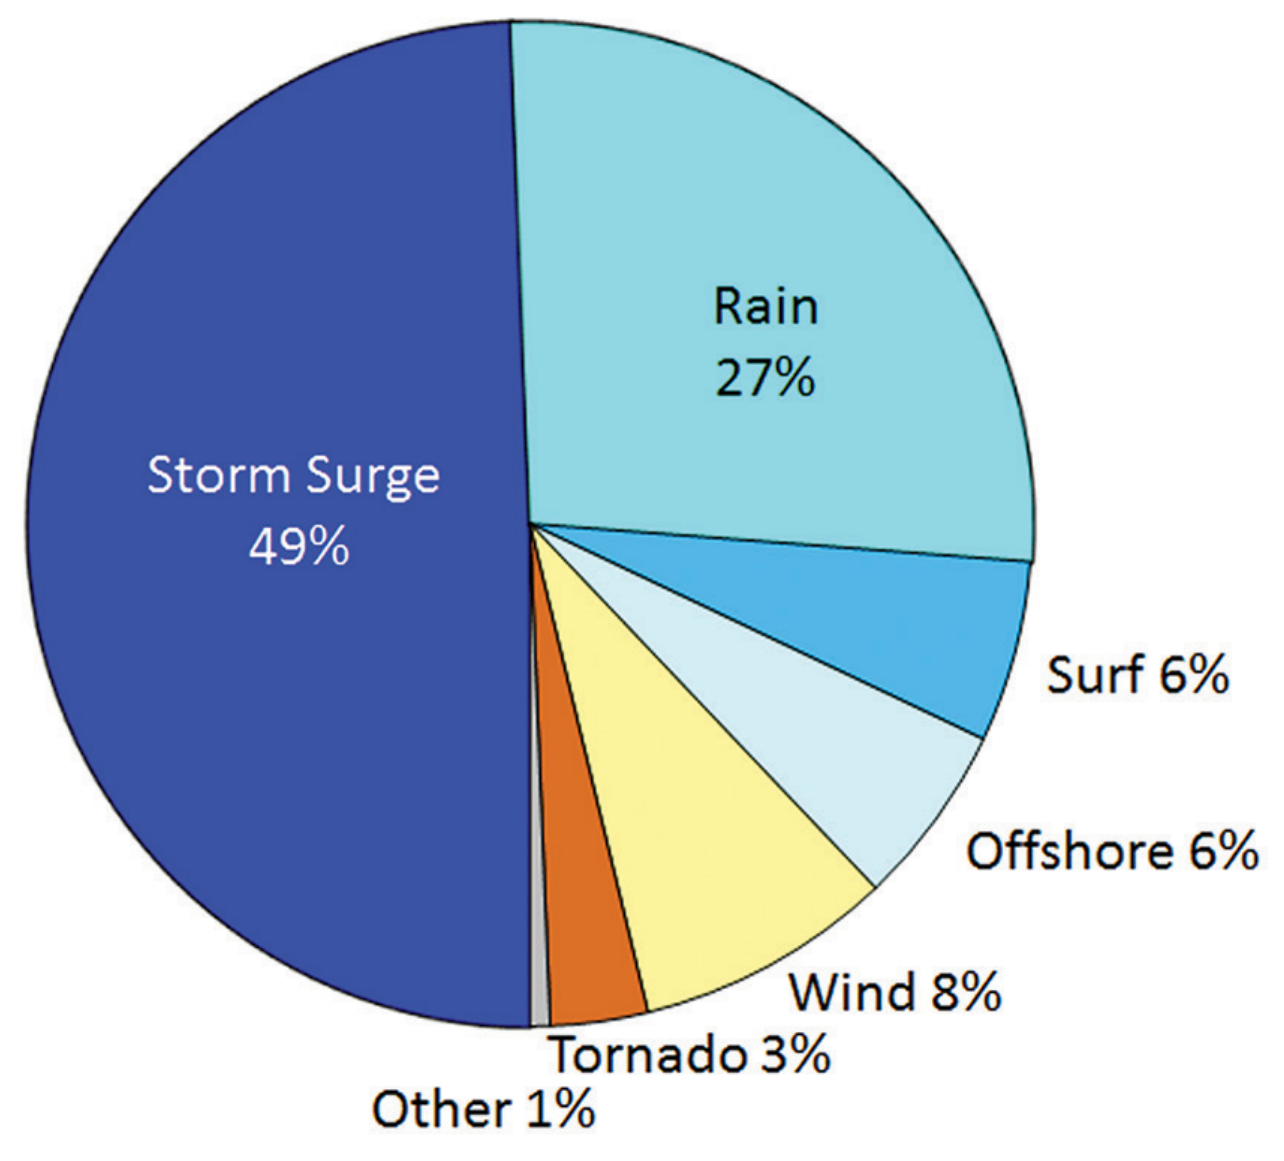
\includegraphics[width=0.6\linewidth]{Deaths}
			\end{tikzfigure}
		}
		\block{Method}{
			
			
			
		}
		
		\column{0.32}
		\block{Comparison}{
		}
		
		\block{Remarks}{
		}
		
		\block{Acknowledgements}{
		}
		
		\block{References}{
			\vspace{-1em}
			\begin{footnotesize}
				\bibliography{refs}
			\end{footnotesize}
		}
	\end{columns}
\end{document} 
